% Created 2013-02-13 Wed 17:46
\documentclass[bigger]{beamer}
\usepackage[utf8]{inputenc}
\usepackage[T1]{fontenc}
\usepackage{fixltx2e}
\usepackage{graphicx}
\usepackage{longtable}
\usepackage{float}
\usepackage{wrapfig}
\usepackage{soul}
\usepackage{textcomp}
\usepackage{marvosym}
\usepackage{wasysym}
\usepackage{latexsym}
\usepackage{amssymb}
\usepackage{hyperref}
\tolerance=1000
\titlegraphic{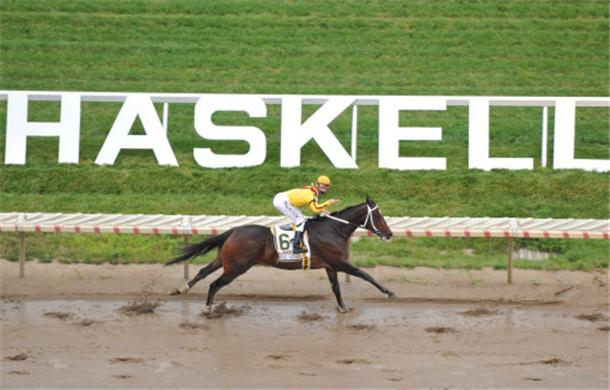
\includegraphics{../pictures/haskell_horse.jpg}}
\setbeamertemplate{navigation symbols}{}
\mode<beamer>{\usetheme{CambridgeUS}}
\institute[GWU]{The George Washington University}
\usepackage{listings}
\lstset{language=Haskell, basicstyle=\scriptsize}
\newcommand{\todo}[1] {\textit{[[TODO: #1]]}}
\providecommand{\alert}[1]{\textbf{#1}}

\title{90\% Demonstration}
\author{Andrew Hirsch}
\date{Thursday, January 17, 2013 }
\hypersetup{
  pdfkeywords={},
  pdfsubject={},
  pdfcreator={Emacs Org-mode version 7.8.11}}

\begin{document}

\maketitle


\begin{frame}
\frametitle{Business issues}
\label{sec-1}



\includegraphics[scale=0.25]{../pictures/business.jpg}

\begin{itemize}
\item Two businesses want to make a deal
\item What needs to happen?
\begin{itemize}
\item Negotiate a deal
\item Sign the paperwork
\end{itemize}
\item What can be bad?
\begin{itemize}
\item Misunderstandings can be devastating
\item Nothing should be binding until the paperwork is filled
\end{itemize}
\end{itemize}
\end{frame}
\begin{frame}
\frametitle{Communication is key}
\label{sec-2}


\begin{itemize}
\item How do businesses make sure nothings wrong?
\end{itemize}

\pause

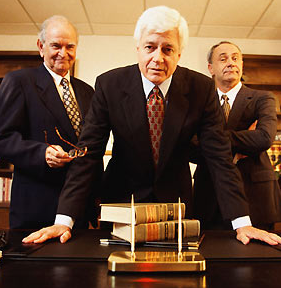
\includegraphics[scale=0.5]{../pictures/lawyer.png}

\begin{itemize}
\item They use lawyers
\item Lawyers know how to speak to each other
\begin{itemize}
\item Makes bad things happen less often
\end{itemize}
\end{itemize}
\end{frame}
\begin{frame}
\frametitle{Communication among thieves (well, lawyers)}
\label{sec-3}



\includegraphics{../pictures/law-book-gavel.jpg}

\begin{itemize}
\item Lawyers need to make misunderstandings not happen
\item Use appropriate protocols
\item Now, everyone knows what that means!
\item Companies do not talk without going through lawyers
\end{itemize}
\end{frame}
\begin{frame}
\frametitle{Now you've gone and put your foot in it}
\label{sec-4}


\includegraphics[scale=0.1]{../pictures/oops.jpg}
\begin{itemize}
\item What happens when things DO go wrong?
\end{itemize}
\pause
\begin{itemize}
\item In come the lawyers again
\item The lawyers can come in and fix the mistake
\item Hopefully, the other businesses don't even notice \\ (These lawyers aren't the most moral sort)
\end{itemize}
\end{frame}
\begin{frame}[fragile]
\frametitle{What on earth has this got to do with computers?}
\label{sec-5}

\begin{itemize}
\item Now you know my opinions on lawyers
\item Let's get down to senior design
\item Working in the \verb~Composite~ operating system
\item \verb~Composite~ has different independent parts, \emph{components}
\item These are like the businesses from that last example.
\end{itemize}
\end{frame}
\begin{frame}
\frametitle{So that was just bias against lawyers?}
\label{sec-6}

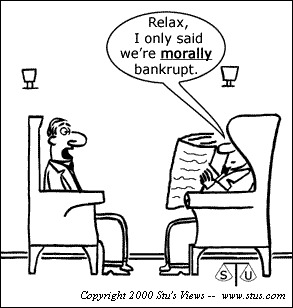
\includegraphics[scale=0.25]{../pictures/morally_bankrupt.jpg}
\begin{itemize}
\item Where do the lawyers come in to this?
\item The components need to be able to talk with each other
\item Things shouldn't go wrong
\item If they do, they should go right again
\item No other components should notice!
\end{itemize}
\end{frame}
\begin{frame}
\frametitle{So about that project\ldots{}}
\label{sec-7}

\begin{itemize}
\item I'm building the lawyers
\end{itemize}

\includegraphics[scale=0.35]{../pictures/building_lawyers.jpg}
\begin{itemize}
\item Lawyers = \emph{stubs}: Code that allows components to talk
\item Before: stubs are generated by hand
\item Now: generated automatically
\end{itemize}
\end{frame}
\begin{frame}
\frametitle{Automatic lawyer machine}
\label{sec-8}

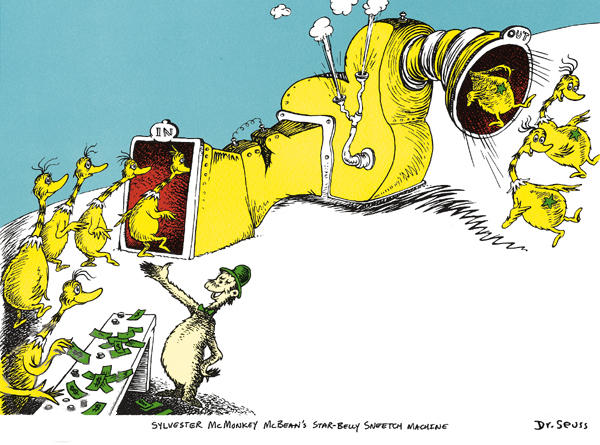
\includegraphics[scale=0.75]{../pictures/star-bellied.jpg}
\begin{itemize}
\item In composite, every component implements an \emph{interface}
\item This specifies what they can do as a list of functions
\item Every function has a stub generated for it
\item This project: language for describing interfaces:\\ \emph{IDL}:  Interface Description Language \\ (Such a creative name, I know)
\end{itemize}
\end{frame}
\begin{frame}
\frametitle{How do lawyers talk to each other?}
\label{sec-9}

\begin{itemize}
\item Every interface also describes a \emph{protocol}
\end{itemize}
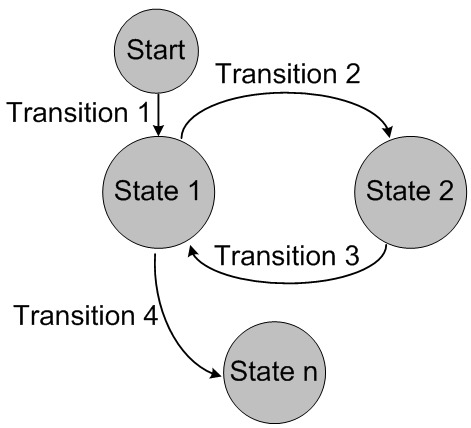
\includegraphics[scale=0.25]{../pictures/fsm.jpg}
\begin{itemize}
\item Protocols can be thought of as how components communicate
\item Similar to the protocols lawyers use
\item These are also described in the IDL \\ (So it's not so uncreatively named after all!)
\end{itemize}
\end{frame}
\begin{frame}
\frametitle{Cleaning up the messes}
\label{sec-10}

\begin{itemize}
\item What happens when a component fails?
\item It should ``un-fail''
\item Other components shouldn't notice!
\item Understand what others expect it to
\item Back to the same spot in IDL protocols
\item Code generated automatically!
\end{itemize}
\end{frame}
\begin{frame}
\frametitle{Demonstration}
\label{sec-11}

\todo{Video here}
\end{frame}

\end{document}
